\chapter{Counterfactuals supplementary}\label{chap:interpretability_appendix}

\begin{figure}[htbp]
    \centering
    \begin{subcaptiongroup}
        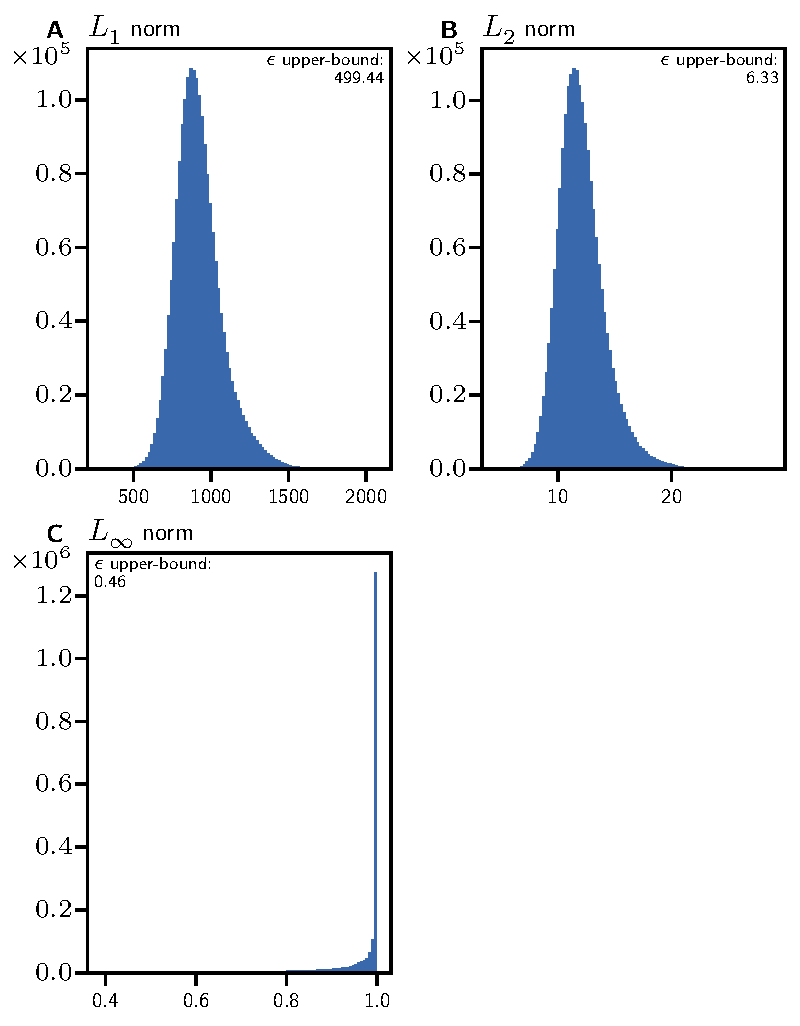
\includegraphics{distance_distribution_classes.pdf}
        \phantomcaption\label{fig:dist_cls_distibutionL1}
        \phantomcaption\label{fig:dist_cls_distibutionL2}
        \phantomcaption\label{fig:dist_cls_distibutionLiinf}
    \end{subcaptiongroup}
    \caption{Distances distributions of points in two different classes}\label{fig:dist_cls_distibution}
\end{figure}

\begin{figure}[htbp]
    \centering
    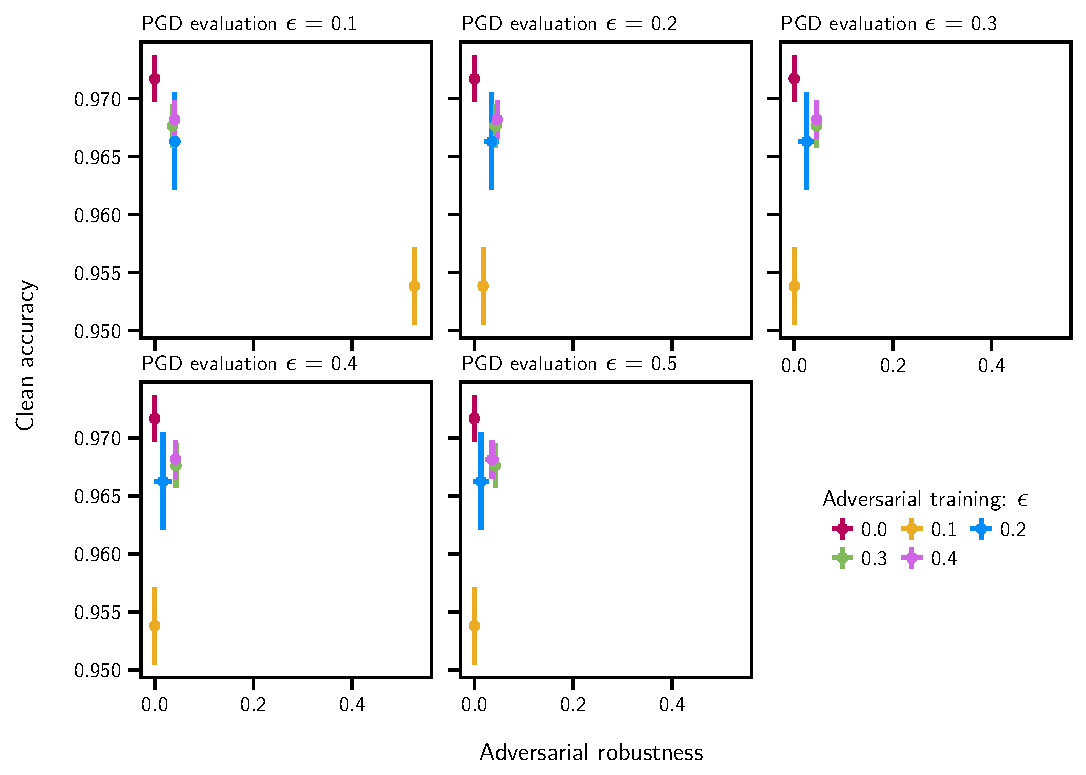
\includegraphics{MLP_LN_adversarial_tradeoff.pdf}
    \caption{<caption>}\label{fig:mlp_ln_adv_tradeoff}
\end{figure}

\begin{figure}[htbp]
    \centering
    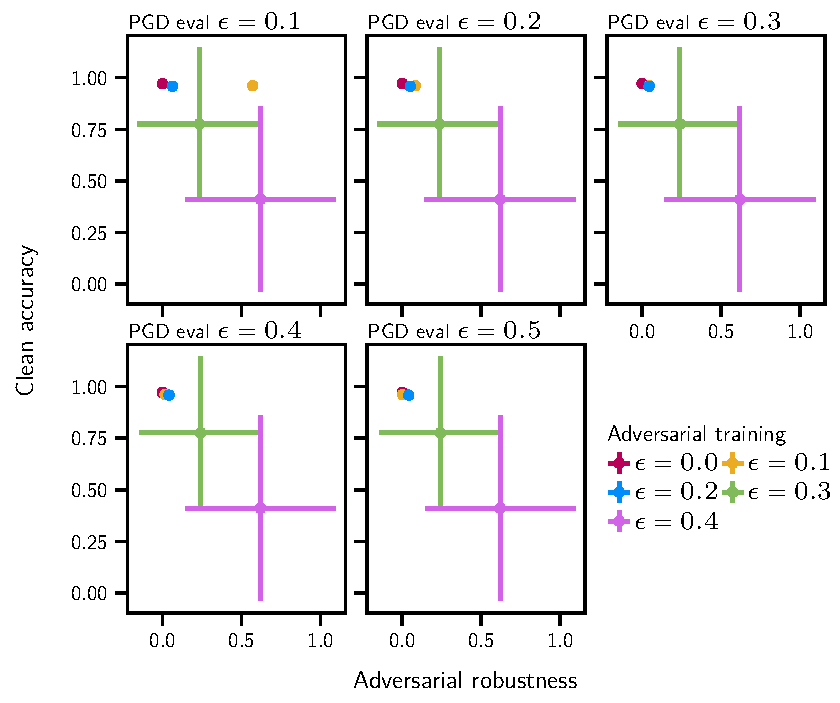
\includegraphics{MLP_NoNorm_adversarial_tradeoff.pdf}
    \caption{<caption>}\label{fig:mlp_nonorm_adv_tradeoff}
\end{figure}

\begin{figure}[htbp]
    \centering
    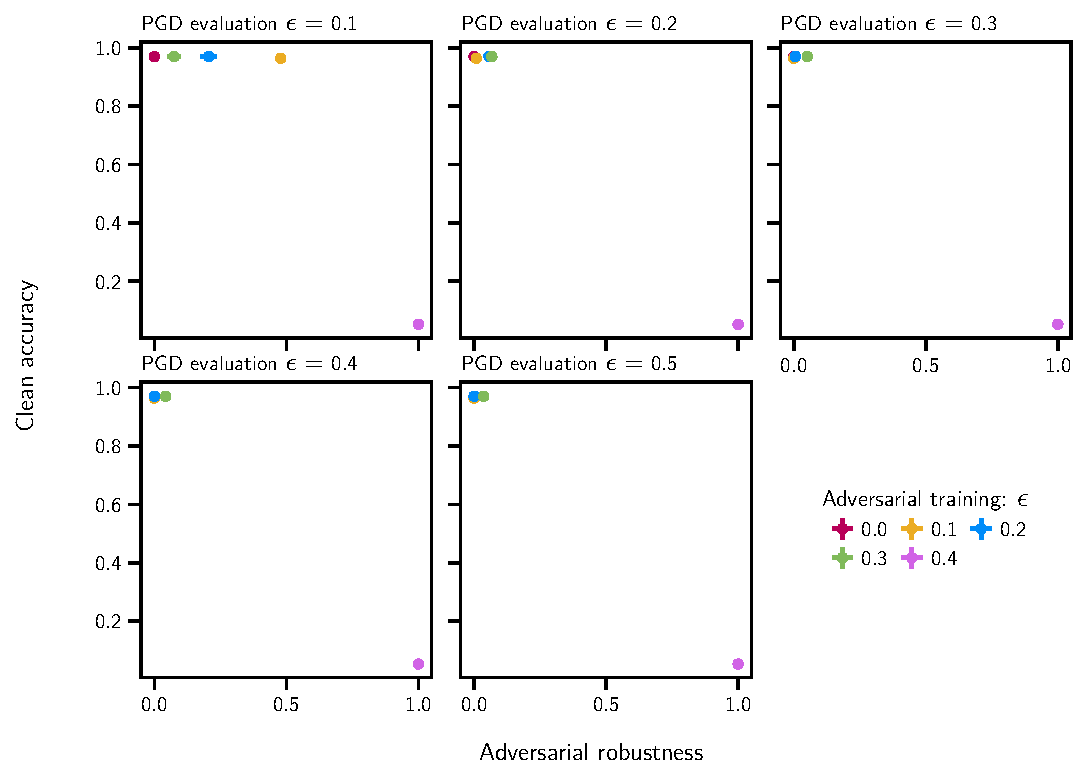
\includegraphics{MLP_FN_adversarial_tradeoff.pdf}
    \caption{<caption>}\label{fig:mlp_fn_adv_tradeoff}
\end{figure}

\begin{figure}[htbp]
    \centering
    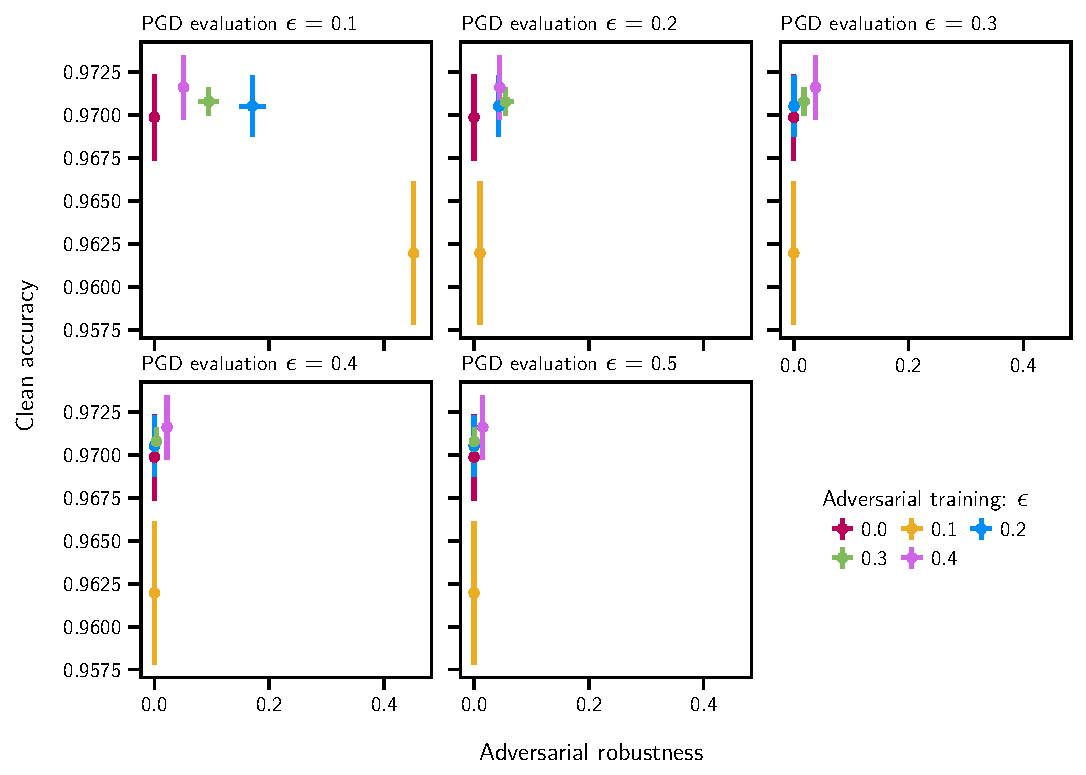
\includegraphics{MLP_FN_AGC_adversarial_tradeoff.pdf}
    \caption{<caption>}\label{fig:mlp_fnagcadv_tradeoff}
\end{figure}

\begin{landscape}
    \begin{figure}[htbp]
        \centering
        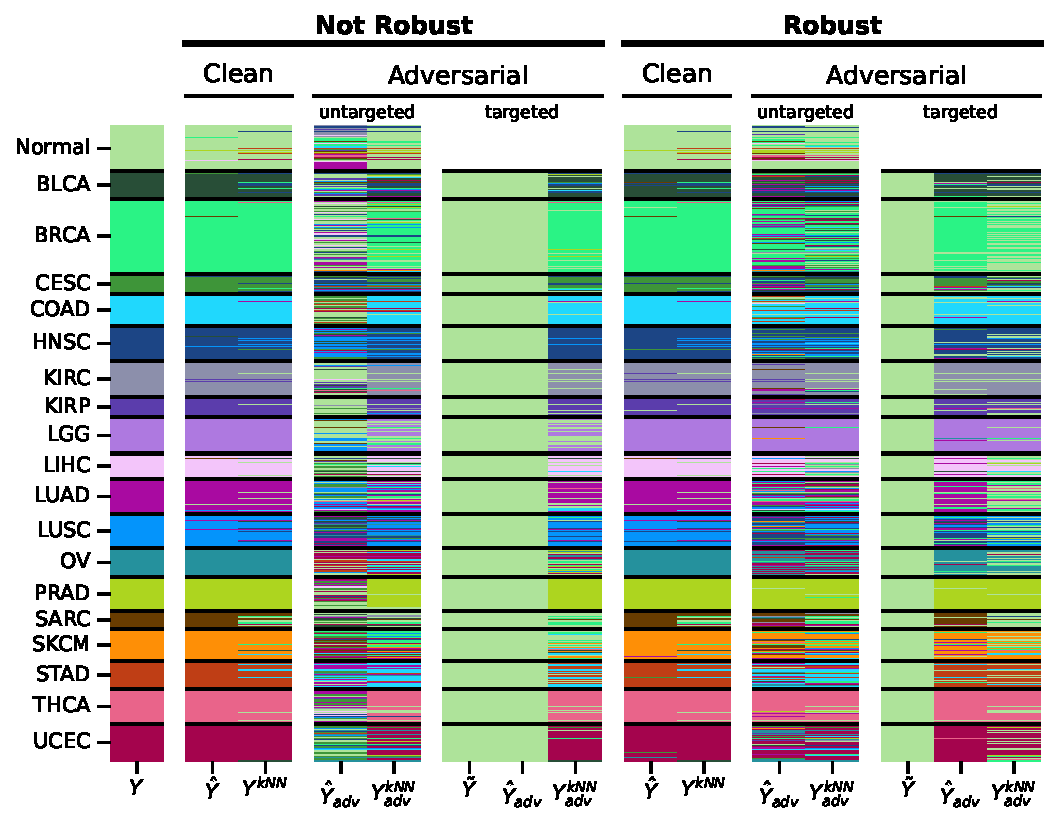
\includegraphics{MLP_LN_knn_comparison.pdf}
        \caption{<caption>}\label{fig:mlp_ln_knn_comp}
    \end{figure}

    \begin{figure}[htbp]
        \centering
        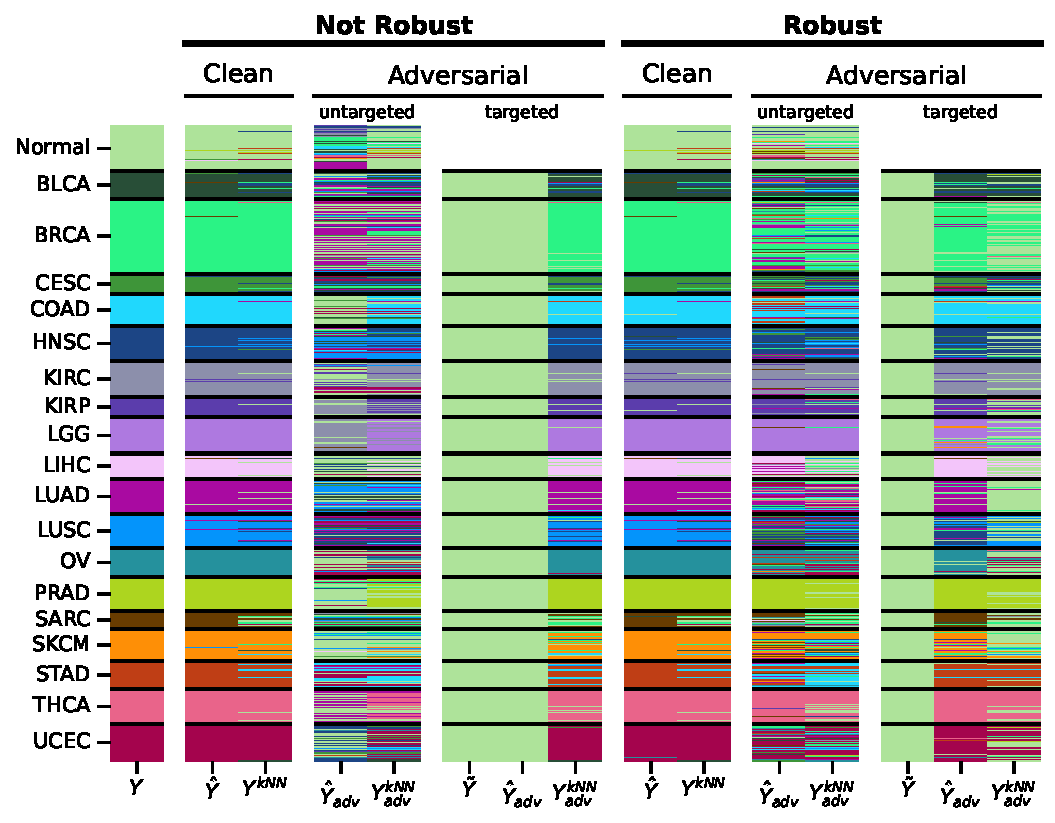
\includegraphics{MLP_NoNorm_knn_comparison.pdf}
        \caption{<caption>}\label{fig:mlp_nonorm_knn_comp}
    \end{figure}

    \begin{figure}[htbp]
        \centering
        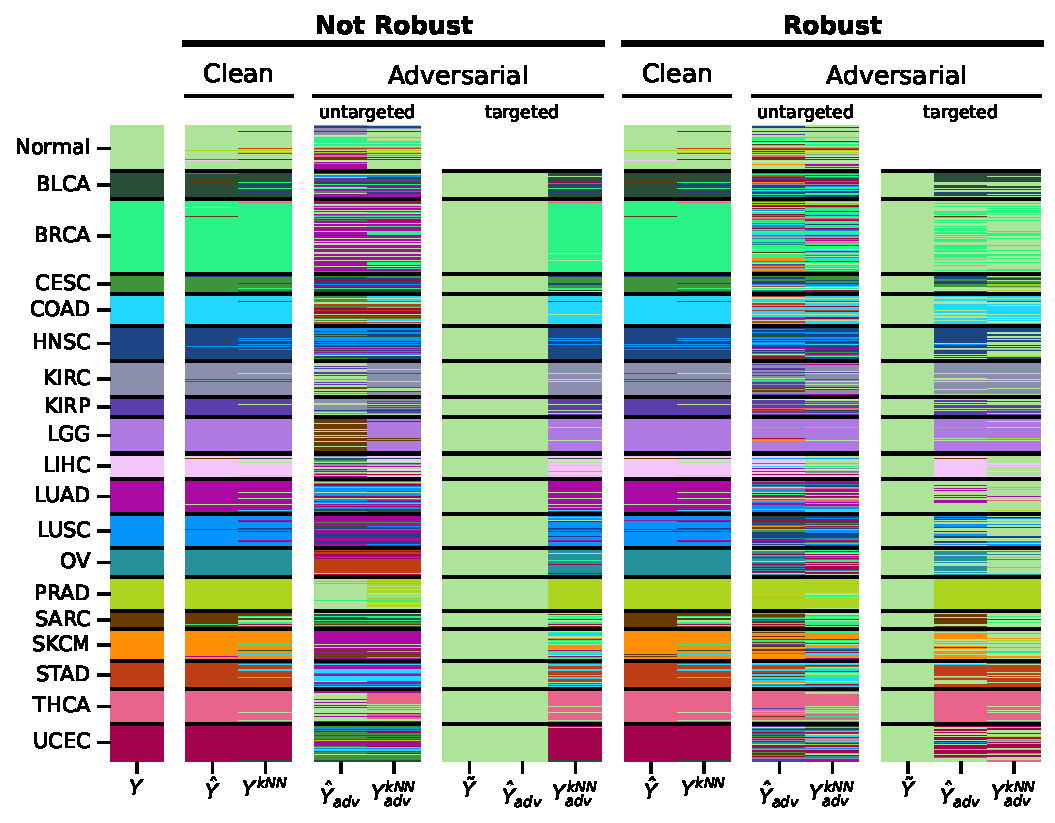
\includegraphics{MLP_FN_knn_comparison.pdf}
        \caption{<caption>}\label{fig:mlp_fn_knn_comp}
    \end{figure}

    \begin{figure}[htbp]
        \centering
        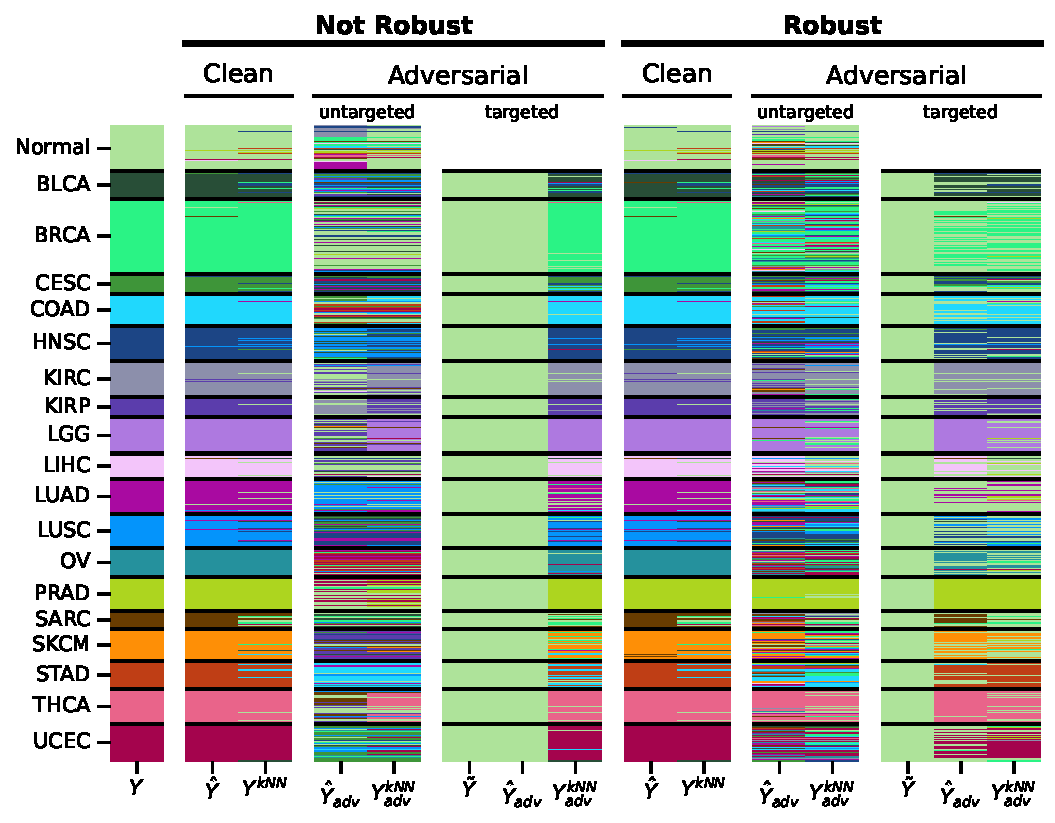
\includegraphics{MLP_FN_AGC_knn_comparison.pdf}
        \caption{<caption>}\label{fig:mlp_fnagc_knn_comp}
    \end{figure}
\end{landscape}